\documentclass[fleqn,10pt]{wlscirep}

% Packages
\usepackage[super]{nth}
\usepackage{rotating}
\usepackage{makecell}
\usepackage{pifont}
\usepackage{amsfonts}
\usepackage{amsmath}
\usepackage{float}
\usepackage{pgfplots}

\pgfplotsset{compat=newest}

% New Commands
\newcommand{\cmark}{\ding{51}}%
\newcommand{\xmark}{\ding{55}}%
\newcommand{\code}[1]{\texttt{#1}}

\title{SciPy 1.0---Fundamental Algorithms for Scientific Computing in Python}

\author[1]{Pauli Virtanen}
\author[2,*]{Ralf Gommers}
\author[3,4]{Tyler Reddy}
\author[5]{Anne Archibald}
\author[6]{Andrew Nelson}
\author[7]{Charles Harris}
\author[8]{CJ Carey}
\author[9]{Denis Laxalde}
\author[10]{Eric Larson}
\author[11]{Eric Moore}
\author[12]{Eric Quintero}
\author[13]{Evgeni Burovski}
\author[14]{Jaime Fernández del Río}
\author[15]{Josef Perktold}
\author[16]{Josh Wilson}
\author[17]{Matthew Brett}
\author[18]{Nikolay Mayorov}
\author[19]{Warren Weckesser}
\author[20]{Matt Haberland}
\author[21]{Scott Sievert}
\author[22]{Yu Feng}
\author[23]{Antonio Horta Ribeiro}

\affil[1]{Affiliation, department, city, postcode, country}
\affil[2]{Affiliation, department, city, postcode, country}
\affil[2]{Affiliation, department, city, postcode, country}
\affil[3]{UC Berkeley Institute for Data Science,
          Berkeley, CA, 94720, USA}
\affil[4]{Los Alamos National Laboratory,
	  Theoretical Division 6,
          Los Alamos, NM, 87545, USA}
\affil[5]{Affiliation, department, city, postcode, country}
\affil[6]{Affiliation, department, city, postcode, country}
\affil[7]{Affiliation, department, city, postcode, country}
\affil[8]{Affiliation, department, city, postcode, country}
\affil[9]{Affiliation, department, city, postcode, country}
\affil[10]{Affiliation, department, city, postcode, country}
\affil[11]{Affiliation, department, city, postcode, country}
\affil[12]{Affiliation, department, city, postcode, country}
\affil[13]{Affiliation, department, city, postcode, country}
\affil[14]{Affiliation, department, city, postcode, country}
\affil[15]{Affiliation, department, city, postcode, country}
\affil[16]{Affiliation, department, city, postcode, country}
\affil[17]{Affiliation, department, city, postcode, country}
\affil[18]{Affiliation, department, city, postcode, country}
\affil[19]{Affiliation, department, city, postcode, country}
\affil[20]{Affiliation, department, city, postcode, country}
\affil[21]{Affiliation, department, city, postcode, country}
\affil[22]{Affiliation, department, city, postcode, country}
\affil[23]{Affiliation, department, city, postcode, country}

\affil[*]{ralf.gommers@gmail.com}

\keywords{Scientific computing, Python, Mathematics}

% NOTE: some usage stats below are from https://libraries.io/pypi/scipy
% as well as github metrics; normally one doesn't put citations directly
% in abstract though (depends on field / journal)
\begin{abstract}
SciPy is an open source scientific computing library for the Python programming language.
SciPy 1.0 was released in late 2017, about 16 years after the original
version 0.1 release. SciPy
has become a \emph{de facto} standard for leveraging scientific algorithms
in the Python programming language, with more than 600
unique code contributors, millions of downloads per year, 161 dependent
packages, and 28700 dependent respositories.
The library includes functionality spanning clustering, Fourier transforms,
integration, interpolation, file I/O, linear algebra, image processing,
orthogonal distance regression, minimization algorithms, signal processing,
sparse matrix handling, computational geometry, and statistics. In this
work, we provide an overview of the capabilities and development practices of the
SciPy library and highlight some recent technical developments.
\end{abstract}
\begin{document}

\flushbottom
\maketitle
\thispagestyle{empty}

\section*{Introduction}

\textit{The Introduction section expands on the background of the work (some overlap with the Abstract is acceptable). The introduction should not include subheadings.}

\textbf{History}

\textbf{Project goals and scope}

\textbf{Current status (maturity, users)}


\section*{Architecture and implementation choices}

\subsection*{Submodule organisation}
The SciPy library is organized as a collection of subpackages.  The 16
subpackages include mathematical building blocks (e.g. linear algebra, Fourier
transforms, special functions), data structures (e.g. sparse matrices, $k$-D trees),
algorithms (e.g. numerical optimization and integration, clustering, interpolation,
graph algorithms, computational geometry), and higher-level data analysis
functionality (e.g. signal and image processing, statistical methods).

Here we summarize the scope and capabilities of each subpackage.

\begin{description}[leftmargin=!, labelwidth=\widthof{\bfseries \texttt{interpolate}}]
\itemsep0em
\item[\texttt{cluster}]
    The \texttt{cluster} subpackage contains two modules:
    \texttt{cluster.vq} provides vector quantization and $k$-means algorithms,
    and \texttt{cluster.hierarchy} provides functions for hierarchical and
    agglomerative clustering.
\item[\texttt{constants}]
    Physical and mathematical constants, including the CODATA recommended
    values of the fundamental physical constants\cite{CODATA2014}.
\item[\texttt{fftpack}]
    Fast Fourier Transform routines.  In addition to the FFT itself, the subpackage
    includes functions for the discrete sine and cosine transforms and for
    pseudo-differential operators.
\item[\texttt{integrate}]
    The \texttt{integrate} subpackage provides tools for the numerical
    computation of single and multiple definite integrals and for the
    solution of ordinary differential equations, including initial value
    problems and two-point boundary value problems.
\item[\texttt{interpolate}]
    The \texttt{interpolate} subpackage contains spline functions and
    classes, one-dimensional and multi-dimensional (univariate and
    multivariate) interpolation classes, Lagrange and Taylor polynomial
    interpolators, and wrappers for FITPACK and DFITPACK functions.
\item[\texttt{io}]
    A collection of functions and classes for reading and writing MATLAB, IDL,
    Matrix Market, Fortran, NetCDF, Harwell-Boeing, WAV and ARFF data files. 
\item[\texttt{linalg}]
    Linear algebra functions, including:
    elementary functions of a matrix, such as the trace, determinant, norm and
    condition number;
    basic solver for $Ax = b$;
    specialized solvers for Toeplitz matrices, circulant matrices, triangular
    matrices and other structured matrices; least squares solver and
    pseudo-inverse calculations; eigenvalue and eigenvector calculations
    (basic and generalized); matrix decompositions, including Cholesky, Schur,
    Hessenberg, $LU$, $LDL^{\intercal}$, $QR$, $QZ$, singular value, and polar;
    and functions to create specialized matrices, such as diagonal, Toeplitz,
    Hankel, companion, Hilbert, and more.
\item[\texttt{ndimage}]
    This package contains various functions for multi-dimensional image
    processing, including convolution and assorted linear and nonlinear
    filters (Gaussian filter, median filter, Sobel filter, etc.);
    interpolation; region labeling and processing; and mathematical morphology
    functions.
\item[\texttt{misc}]
    A collection of functions that did not fit into the other subpackages.
    While this subpackage still exists in SciPy 1.0, effort is underway
    to deprecate or relocate the contents of this subpackage and eventually remove it.
\item[\texttt{odr}]
    Orthogonal distance regression, including Python wrappers for the Fortran
    library ODRPACK.
\item[\texttt{optimize}]
    The package includes the following, with additional details in the SI:
    simplex and interior-point linear programming solvers,
		implementations of many nonlinear minimization algorithms,  
		a routine for least-squares curve fitting, and 
		a collection of general nonlinear solvers for root-finding.
\item[\texttt{signal}]
    The \texttt{signal} subpackage focuses on signal processing and
    basic linear systems theory.  Functionality includes
    convolution and correlation; splines; filtering and filter design;
    continuous and discrete time linear systems; waveform generation;
    window functions; wavelet computations; peak finding; and spectral
    analysis.  
\item[\texttt{sparse}]
    This package includes implementations of several representations of
    sparse matrices.  It contains two modules, 
    \texttt{scipy.sparse.linalg} and \texttt{scipy.sparse.csgraph}.

    \texttt{scipy.sparse.linalg} provides a collection of linear algebra
    routines that work with sparse matrices, including linear equation
    solvers, eigenvalue decomposition, singular value decomposition
    and LU factorization.

    \texttt{scipy.sparse.csgraph} provides a collections of graph algorithms
    for which the graph is represented using a sparse matrix.  Algorithms
    include connected components, shortest path, minimum spanning tree
    and more.
\item[\texttt{spatial}]
    This subpackage provides spatial data structures and algorithms,
    including the $k$-d tree, Delaunay triangulation, convex hulls and Voronoi
    diagrams.  The subpackage \texttt{scipy.spatial.distance} provides
    a large collection of distance functions, along with functions for
    computing the distance between all pairs of vectors in a given collection
    of points or between all pairs from two collections of points.
\item[\texttt{special}]
    The name comes the class of functions traditionally known as \emph{special
    functions}, but over time, the subpackage has grown to include functions
    beyond the classical special functions.  A more appropriate characterization
    of this subpackage is simply \emph{useful functions}.
    It includes a large collection of the classical special functions
    such as Airy, Bessel, etc.; orthogonal families of polynomials;
    the Gamma function, and functions related to it;
    functions for computing the PDF, CDF and quantile function for several
    probability distributions;
    information theory functions;
    combinatorial functions \texttt{comb} and \texttt{factorial};
    and more.
\item[\texttt{stats}]
    The \texttt{stats} subpackage provides a large collection of continuous
    and discrete \emph{probability distributions}, each with methods to compute
    the PDF or PMF, CDF, moments and other statistics, generation of random
    variates, and more;
    \emph{statistical tests}, including Pearson's correlation, Spearman's rank-order
    correlations, Kendall's tau, chi-squared test and its generalization as the
    Cressie-Read power divergence, contingency table tests including Fisher's
    exact test and Mood's median test, and many more;
    and assorted \emph{transformations and statistics} of data.
\end{description}


\subsection*{Common infrastructure}

\subsection*{Language choices}
Python, Cython, Fortran, C and C++ are the programming languages
used to implement scientific algorithms in the SciPy library. An analysis
of our code base using the \texttt{linguist} library provides a detailed
breakdown as \% composition by programming language in SciPy
(Figure~\ref{fig:linguist}).

    \begin{figure}[H]
        \centering

        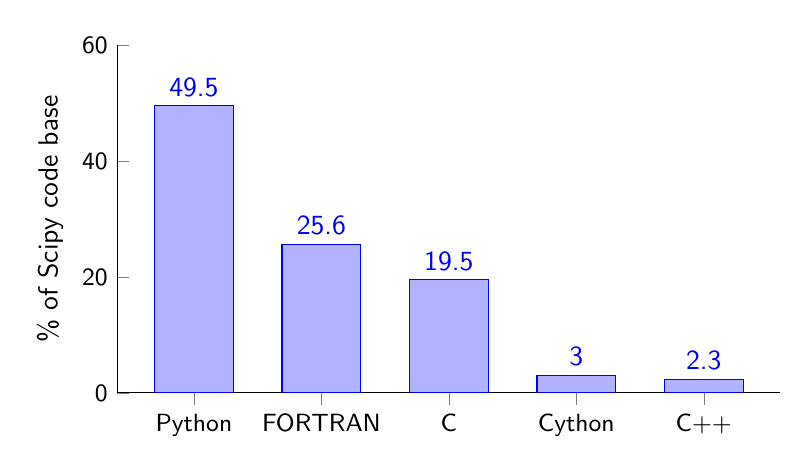
\begin{tikzpicture}[font=\sffamily]
        \begin{axis}[height=6cm, width=10cm,
        ybar, ymax=60, ymin=0,bar width=1cm,
        ylabel={\% of Scipy code base},
        ytick={0,20,...,60},
        axis lines*=left,
        axis y line shift=0pt,
        enlarge x limits=0.15,
        symbolic x coords={py,f,c,cy,cpp},
        xticklabels={Python,FORTRAN,C,Cython,C++},
        ticklabel style={align=center,font=\sffamily\small,
        /pgf/number format/assume math mode=true},
        xtick=data,
        nodes near coords,
        nodes near coords style={/pgf/number format/assume math mode=true}
        ]
        \addplot coordinates {(py,49.5) (f,25.6) (c,19.5) (cy, 3.0) (cpp,2.3)};
        \end{axis}
        \end{tikzpicture}
        \caption{The breakdown of programming languages used in the
	         SciPy library determined using the linguist library.
		 Small ($<0.5 \%$) amounts of TeX, Matlab, Shell,
		 and Makefile are excluded for clarity and mostly
		 provide supporting roles in tests, building, and
		 documentation.}
        \label{fig:linguist}
    \end{figure}

For implementing new functionality, we have a clear order of language preference.
First Python, if performance is not an issue. If it is, then in order of
preference: Cython, C, C++, Fortran. The main motivation for this is 
maintainability: Cython has the highest abstraction level and most 
Python developers will understand it. C is also widely known,
and easier to deal with for the core development team
than C++ and especially Fortran.

While it is not surprising that Python is heavily used in SciPy, the
usage distribution of the other languages warrants some discussion. Fortran
is an extremely well-established scientific programming language, both
for historical reasons and because of its continued excellent
performance\cite{Koelbel:1993:HPF:562354}. We
wrap the FFTPACK Fortran library for performing Fourier
transforms\cite{SWARZTRAUBER198445, SWARZTRAUBER198251} since
this library has been a standard in the field for 33 years and has a license
that is compatible with our own. Likewise, we wrap the Fortran source
for ODEPACK\cite{citeulike:2644528} as it has been  trusted for the initial 
value problem for ordinary differential equation systems for 30 years. For
similar reasons we also wrap the Fortran libraries QUADPACK\cite{1983qspa.book.....P} (for numerical
integration of one-dimensional functions), FITPACK\cite{Dierckx:1993:CSF:151103} (curve-fitting /
interpolation), ODRPACK\cite{ODRPACK_Boggs} (orthogonal distance regression),
MINPACK\cite{osti_6997568} (minimization of linear and nonlinear equations),
ARPACK\cite{leh:sor:yan96} (solving large scale eigenvalue problems), 
ALGORITHM 644\cite{Amos:1986:APP:7921.214331} (handling Bessel Functions), and 
CDFLIB\cite{CDFLIB_site} (evaluation of cumulative density functions).

Rounding out the top three languages in SciPy is C, which is also extremely
well-established over several decades\cite{Kernighan:1988:CPL:576122} of
scientific computing. Alongside its objected-oriented relative C++, C
can be leveraged in Python after being exposed using the Cython
language. Cython has been described as a creole language that mixes
the best parts of Python and lower-level C / C++
paradigms\cite{behnel2011cython}. We thus often use Cython as a glue
between well-established low-level scientific computing libraries and
the Python interface offered by SciPy. We also use Cython to enable
performance enhancements in Python code, especially for cases where heavily
used inner loops benefit from a compiled code with static typing. Some of the C
libraries that we wrap in SciPy include trlib\cite{doi:10.1080/10556788.2018.1449842} 
(iterative solving of the trust region problem), SuperLU\cite{li05,superlu_ug99} (solution of
large, sparse, nonsymmetric systems of linear equations),
Qhull\cite{Barber:1996:QAC:235815.235821} (computational
geometry), and Cephes\cite{cephes_netlib} (mathematics algorithms). 

Therefore, the relative abundance of different programming languages
in the SciPy library results from a combination of the usage of powerful performance
enhancing languages that interact well with Python (i.e., Cython), and
the usage of languages (and their libraries) that have proven reliable
and performant over many decades. The position that SciPy occupies
near the foundation of the scientific Python ecosystem is such that
adoption of new languages or major dependencies is generally unlikely--our
choices are strongly driven by long-term stability. GPU acceleration,
new transpiling libraries, and the latest JIT compilation approaches
(i.e., Numba\cite{Lam:2015:NLP:2833157.2833162}) are very powerful, but currently fall outside the remit
of the main SciPy library. That said, we have recently increased our
efforts to support compatibility with some of these options, and having
our full test suite pass with the PyPy JIT compiler\cite{Bolz:2009:TMP:1565824.1565827}
is now a requirement in our development workflow.

\subsection*{API and ABI evolution}


\section*{Key technical improvements}

Here we describe key technical improvements made in the last three years.

\subsection*{Data structures}
\textbf{cKDTree}
The \texttt{cKDTree} module, which implements a space-partitioning data structure that
organizes points in $k$-dimensional space, was rewritten in C++ with templated classes. 
Support was added for periodic boundary conditions, which are often used 
in simulations of physical processes. 

In 2013, the time complexity of the $k$-nearest neighbor search from
\texttt{cKDTree.query} was approximately loglinear \cite{knn-jake},
consistent with its formal description \cite{kdtree-search-algo}.
Since then, we've enhanced \texttt{cKDTree.query} by reimplementing it in
C++, removing memory leaks, and allowing release of the global interpreter lock (GIL) so that
multiple threads may be used\cite{gh-4374}. This generally improved
performance on any given problem (Figure~\ref{fig:asvbench}) while
preserving the asymptotic complexity (Figure~\ref{fig:knn-complexity}).

In 2015, SciPy added the \texttt{sparse\_distance\_matrix} routine for generating 
approximate sparse distance matrices between \texttt{KDTree} objects by ignoring 
all distances that exceed a user-provided value. Also, this routine is not 
limited to the conventional L2 (Euclidean) norm but supports any Minkowski 
p-norm between 1 and infinity. By default, the returned data structure is a 
Dictionary Of Keys (DOK) based sparse matrix, which is very efficient for matrix 
construction. This hashing approach to sparse matrix assembly can be 7 times 
faster than constructing with CSR format
\cite{10.1007/978-3-540-75755-9_107}, and the C++ level sparse matrix construction 
releases the Python GIL for increased performance. Once the matrix is constructed, 
distance value retrieval has an amortized constant time complexity 
\cite{Cormen:2001:IA:580470}, and the DOK structure can be efficiently converted 
to a CSR, CSC, or COO matrix to allow for 
speedy arithmetic operations.

In 2015 the \texttt{cKDTree} dual tree counting algorithm\cite{Moore2000ar}
was enhanced to support weights\cite{ckdtree-weights}, which are
essential in many scientific applications, e.g. computing correlation
functions of galaxies\cite{0004-637X-750-1-38}.

\textbf{Sparse matrices}

\subsection*{Unified bindings to compiled code}
\subsubsection*{LowLevelCallable}
As of SciPy version 0.19, it is possible for users to wrap low-level
functions in a \texttt{scipy.LowLevelCallable()} object that reduces
the overhead for calling compiled C functions directly from Python.
Supported low-level functions include \texttt{PyCapsule} objects,
ctypes function pointers, and cffi function pointers. The low level
function signature must be consistent with the expectations of the
routine it is passed to. For example, the documentation for
\texttt{scipy.ndimage.generic\_filter} defines two acceptable C callback
function signatures that may be used to produce functions that operate
on each element of image data with low overhead. The C code may be
generated using numba or Cython, for example, as long as the function
call signature matches the specifications. Furthermore, it is even
possible to generate a low-level callback function automatically
from a Cython module using \texttt{scipy.LowLevelCallable.from\_cython}.

\subsection*{Cython bindings for BLAS, LAPACK and special}

\subsection*{Numerical optimization}
\newcommand{\RR}{\ensuremath{\mathbb{R}}}
The \texttt{scipy.optimize} module provides functions for the numerical solution of several classes of root finding and optimization problems:
\begin{enumerate}
\item nonlinear root finding problems (\texttt{brentq}, \texttt{brenth}, \texttt{ridder}, \texttt{bisect}, \texttt{newton}, and \texttt{root}),
\item linear sum assignment problems (\texttt{linear\textunderscore sum\textunderscore assignment}),
\item linear and nonlinear sum-of-squares problems (\texttt{leastsq}, \texttt{least\textunderscore squares}, \texttt{nnls}, \texttt{lsq\textunderscore linear}, and \texttt{curve\textunderscore fit}),
\item general, linear optimization problems (\texttt{linprog}),
\item general, nonlinear, local optimization problems of a single variable (\texttt{minimize\textunderscore scalar}),
\item general, nonlinear, local optimization problems of several variables (\texttt{minimize}), and
\item general, nonlinear, global optimization problems of several variables (\texttt{basinhopping}, \texttt{brute}, \texttt{differential\textunderscore evolution}).
\end{enumerate}
Documentation of SciPy's functionality in each these areas can be found in (cite SciPy documentation), but here we highlight recent additions through SciPy 1.0.

%\subsubsection{Root Finding}
%The general ``root finding'' problem is to find a root $\mathbf{x} \in \RR^m$ of $\mathbf{f}: \RR^m \rightarrow \RR^m$, that is, to solve
%\begin{equation}
%\mathbf{f}(\mathbf{x}) = \mathbf{0}
%\end{equation}
%for a solution $\mathbf{x}$.\footnote{Equivalently the problem is to simultaneously find the roots $x_i \in \RR$ of several scalar functions $f_i : \RR \rightarrow \RR$, that is, to solve $f_i(x_0, x_1, \dots, x_{m-1}) = 0$ for $x_i$, $i \in \{0, 1, \dots {m-1}\}$.} The function \texttt{scipy.optimize.root} provides a common interface to several algorithms for solving problems of this type. For the special case\footnote{that is, to solve a single scalar equation $f(x) = 0$ for a single scalar variable $x$} $m = 1$, any one of several specialized functions \texttt{brentq}, \texttt{brenth}, \texttt{ridder}, \texttt{bisect}, or \texttt{newton} may provide improved performance or accuracy. (Have there been any recent improvements? Do we want to summarize the methods as @antonior92 has done for $minimize$? Do we have to explain that these methods only provide \emph{one} solution, and that they are iterative based on a user-provided guess? Do we have to explain the notion of tolerance? Is this a good template for the beginning of the following subsections?)


\subsubsection*{Linear Optimization}

A new interior-point optimizer for continuous linear programming problems, \texttt{linprog} with \texttt{method='interior-point'}, was released with SciPy 1.0. Implementing the core algorithm of the commercial solver MOSEK \cite{andersen2000mosek}, it solves all of the 90+ NETLIB LP benchmark problems \cite{netlib} tested. Unlike some interior point methods, this homogenous self-dual formulation provides certificates of infeasibility or unboundedness as appropriate. 

A presolve routine \cite{andersen1995presolving} solves trivial problems and otherwise performs problem simplifications, such as bound tightening and removal of fixed variables, and one of several routines for eliminating redundant equality constraints is automatically chosen to reduce the chance of numerical difficulties caused by singular matrices. Although the main solver implementation is pure Python, end-to-end sparse matrix support and heavy use of SciPy's compiled linear system solvers --- often for the same system with multiple right hand sides due to the predictor-corrector approach --- provide speed sufficient for problems with tens of thousands of variables and constraints.

Compared to the previously implemented simplex method, the new interior-point method is faster for all but the smallest problems, and is suitable for solving medium- and large-sized problems on which the existing simplex implementation fails. However, the interior point method typically returns a solution near the center of an optimal face, yet basic solutions are often preferred for sensitivity analysis and for use in mixed integer programming algorithms. This motivates the need for a crossover routine or a new implementation of the simplex method for sparse problems in a future release, either of which would require an improved sparse linear system solver with efficient support for rank-one updates

\subsubsection*{Nonlinear Optimization}


The \texttt{minimize} function provides methods for solving nonlinear optimization
problems. It unifies several methods with a common interface in order to facilitate
interchanging between solvers with different characteristics, summarized in Table~\ref{tab:minimize}.
%% Currently, this introduces a ton of whitespace around a very simple expression (min f(x)). The reader can easily find the standard of meaning of `nonlinear programming', so I believe it should be removed. If we decide that it is appropriate to include, then we should add the entire problem statement - including constraints - and we should also include the entire linear programming problem statement in the previous section.
% summarizes all the methods available for solving minimization problems of the type:
%\begin{equation}
%  \label{eq:minimization-prob}
%  \min_x f(x)
%\end{equation}
%where $f$ is a multivariate function $f: \mathbb{R}^n \rightarrow \mathbb{R}$ and $x \in \mathbb{R}^n$.
%%  Without the problem statement this sentence isn't really appropriate.
%\texttt{COBYLA} and \texttt{SLSQP} methods support nonlinear constraints, \texttt{L-BFGS-B} and \texttt{TNC} allow box constraints $x^l \le x \le x^u$,
%and the remaining methods are for unconstrained problems.

% The available methods implement a variety of solution strategies.
Derivative-free methods (e.g. \texttt{Nelder-Mead}, \texttt{Powell} and \texttt{COBYLA}) are appropriate for minimizing non-differentiable or
noisy objective functions. When derivatives are available, however, other methods offer faster convergence rates
and have proven convergence properties. 
The derivative-based methods start with an initial guess and refine it iteratively, seeking
a local solution to the optimization problem. Each of these algorithms implements one of two complementary strategies:
line-search or trust-region. At each iteration, the line-search (LS) methods choose a direction
and approximate the optimal point in the given direction. Trust-region (TR) methods, on the other
hand, choose a ``trust-region'' region for which a local model is valid and approximate the best point
inside.

One recently-added trust-region method is \texttt{trust-exact},
which achieves fast convergence by solving the trust-region subproblem almost exactly.
Unfortunately, it requires the Hessian to be stored and factored every iteration, which may preclude
the solution of large problems (e.g.~problems with more than 1000 variables).
Other methods are appropriate for large-scale problems, including
\texttt{CG}, which does not use second derivatives and thus has low memory requirements, and \texttt{L-BFGS-B}, which maintains a simple and compact representation of the Hessian.
\texttt{Newton-CG}, \texttt{trust-ncg} and \texttt{trust-krylov} use second order derivatives to achieve faster
convergence, but are still appropriate for large problems because they factorize the Hessian in an inexact and iterative way that does not require the Hessian to be stored.
The method \texttt{trust-krylov}, introduced in the latest release, is a good compromise between
\texttt{trust-ncg} and \texttt{trust-exact}: it provides a more accurate solution to the trust-region
subproblem than \texttt{trust-ncg}, but it does not require the Hessian to be stored and factored as in \texttt{trust-exact}.

While most \texttt{minimize} development prior to SciPy 1.0 has focused on unconstrained minimization, methods \texttt{SLSQP} and \texttt{COBYLA}\footnote{We note that any equality constraint $c_{\text{eq}}(x) = 0$ can be expressed as two inequality constraints $c_{\text{eq}}(x) \leq 0$ and $-c_{\text{eq}}(x) \leq 0$} support fully general nonlinear programming. However, neither provides special treatment for sparsity. Accordingly, ongoing development efforts for \texttt{minimize} are focused on the addition of nonlinear programming algorithms for large, sparse problems. 

\begin{table}[H]
  \centering
  \caption{Optimization methods from \texttt{minimize}, which solves problems of the form $\min_x f(x)$, where $x \in \mathbb{R}^n$ and $f: \mathbb{R}^n \rightarrow \mathbb{R}$ .  The field \textit{version added} specifies the algorithm's first appearance in SciPy. Algorithms with \textit{version added} ``0.6*'' were added in version 0.6 or before.
    The field \textit{wrapper} indicates whether the implementation available in SciPy wraps a function written in a compiled language
    (e.g. C or FORTRAN). The fields \textit{\nth{1}} and \textit{\nth{2} derivatives}
    indicates whether first or second order derivatives are required. When \textit{\nth{2} derivatives} is flagged
    with $\sim$ the algorithm does not requires second-order derivatives from
    the user; it computes an approximation internally and uses it to accelerate method convergence.
    \textit{Iterative Hessian factorization} denotes algorithms that factorize the Hessian in an iterative way,
    which does not require explicit matrix factorization or storage of the Hessian.
    \textit{Local convergence} gives a lower bound on the rate of convergence of the iterations sequence once the
    iterate is sufficiently close to the solution: linear (L), superlinear (S) and quadratic (Q). Convergence rates denoted S$^*$ indicate that the algorithm
    has a superlinear rate for the parameters used in SciPy, but can  achieve a quadratic convergence rate with other parameter choices.
    \textit{Global convergence} is marked for the algorithms with guarantees of convergence to a stationary
    point (i.e. a point $x^*$ for which $\nabla f(x^*) = 0$). The table also indicates which algorithms
    can deal with constraints on the variables. We distinguish between: \textit{bound constraints} (i.e. $x^l \le x \le x^u$),
    \textit{equality constraints} (i.e. $c_{\text{eq}}(x) = 0$) and \textit{inequality constraints} (i.e. $c_{\text{ineq}}(x) \ge 0$).}
  \begin{tabular}{cccccccccccccc}
      & \rotatebox{80}{\texttt{Nelder-Mead}} & \rotatebox{80}{\texttt{Powell}} & \rotatebox{80}{\texttt{COBYLA}} & \rotatebox{80}{\texttt{CG}} & \rotatebox{80}{\texttt{BFGS}}&  \rotatebox{80}{\texttt{L-BFGS-B}} & \rotatebox{80}{\texttt{SLSQP}} & \rotatebox{80}{\texttt{TNC}} & \rotatebox{80}{\texttt{Newton-CG}} & \rotatebox{80}{\texttt{dogleg}} & \rotatebox{80}{\texttt{trust-ncg}} & \rotatebox{80}{\texttt{trust-exact}} & \rotatebox{80}{\texttt{trust-krylov}} \\
    \hline
    Version added &  0.6* &  0.6* &  0.6* &  0.6* &  0.6* &  0.6* &  0.9 &  0.6* &  0.6* & 0.13 & 0.13 & 0.19 & 1.0 \\
    \hline
    Wrapper & & & \cmark & & & \cmark & \cmark & \cmark & &  & & & \cmark \\
    \hline
    \nth{1} derivatives &  & & & \cmark  & \cmark & \cmark & \cmark & \cmark & \cmark & \cmark & \cmark & \cmark & \cmark \\
    \hline
    \nth{2} derivatives &  &  &  &  & $\sim$ & $\sim$ & $\sim$ & \cmark & \cmark & \cmark & \cmark & \cmark & \cmark \\
    \hline
    \makecell{Iterative Hessian \\
    factorization} & & & &  & & & & \cmark & \cmark &  & \cmark &  & \cmark \\
    \hline
    Local convergence& & & & L & S &  L & S & S$^*$ & S$^*$ & Q & S$^*$ & Q & S$^*$  \\
    \hline
    Global convergence & & &  &   & \cmark & \cmark & \cmark & \cmark & \cmark & \cmark & \cmark & \cmark & \cmark  \\
    \hline
    \makecell{Line-search (LS) or\\ trust-region (TR)} & Neither  & LS &  TR & LS & LS & LS & LS & LS & LS & TR & TR & TR & TR \\
    \hline
    Bound constraints &&&\cmark&&&&\cmark&\cmark&\cmark&&&& \\
    \hline
    Equality constraints &&&&&&&\cmark&&&&& \\
    \hline
    Inequality constraint &&&\cmark&&&&\cmark&&&&& \\
    \hline
    References & \cite{nelder_simplex_1965, wright_direct_1996} & \cite{powell_efficient_1964} &
      \cite{powell_direct_1994, powell_direct_1998, powell_view_2007} &
      \cite{polak_note_1969, nocedal_numerical_2006} & \cite{nocedal_numerical_2006} & \cite{byrd_limited_1995, zhu_algorithm_1997} &
      \cite{schittkowski_nonlinear_1982, schittkowski_nonlinear_1982-1, schittkowski_convergence_1983, kraft_software_1988} &
      \cite{nash_newton-type_1984} & \cite{nocedal_numerical_2006}  & 
      \cite{powell_new_1970, nocedal_numerical_2006} &  \cite{steihaug_conjugate_1983, nocedal_numerical_2006} &
      \cite{conn_trust_2000, more_computing_1983} & \cite{gould_solving_1999, lenders_trlib:_2016} \\
    \hline
  \end{tabular}
  \label{tab:minimize}
\end{table}

Some problems may require the use of global optimizers to find the minimum of the objective function over the set of all parameter values, especially if the objective function possesses many local minima that other solvers could get stuck in.
\texttt{Brute} performs a grid search over the entire parameter range, with the best grid point undergoing further polishing by another solver. However, this approach becomes increasingly inefficient as the problem dimensionality increases, or if the objective function has many extrema.
\texttt{Basinhopping} \cite{Wales1997} uses random perturbation of the parameter vector, with local minimization. The acceptance of the new coordinates is dictated by the Metropolis test typically used in Monte Carlo simulations.
\texttt{differential\textunderscore evolution} \cite{Wormington1999,Storn1997} is a stochastic solver that improves by gradual evolution of a population of candidate solutions. In each iteration trial candidates are generated by combination of candidates from the existing population; if the trial candidates represent an improvement then the population is updated. \texttt{differential\textunderscore evolution} does not require that the objective function be differentiable.
%  basinhopping may need differentiable objective for the local minimization.
The SciPy benchmark suite possesses a comprehensive range of global optimization problems (196), of varying difficulties, that can be used to evaluate the performance of a particular solver. This suite is used to decide whether new solvers have good enough performance to be added to the package.


\subsection*{Statistical distributions}

%%%%%%%%%%%%%%%%%%%%%%%%%%%%%
\subsection*{Polynomial interpolators}
Traditionally, SciPy relied heavily on the venerable \texttt{FITPACK}
Fortran library by P.~Dierckx \cite{Dierckx:1993:CSF:151103, FITPACK} for
univariate interpolation and approximation of data. The original monolithic
design and API for interaction between SciPy and FITPACK was limiting for both
users and developers, as detailed in the Supporting Information.

Implementing a new, modular design of polynomial interpolators was spread over
several releases. The goals of this effort were to have a set of basic objects
representing piecewise polynomials, to implement a collection of algorithms
for constructing various interpolators, and to provide users with building
blocks for constructing additional interpolators.

At the lowest level of the new design are classes which represent univariate
piecewise polynomials: \code{PPoly} (SciPy 0.13)\cite{scipy-gh2885},
\code{BPoly} (SciPy 0.13) and \code{BSpline} (SciPy 0.19)\cite{scipy-gh3174},
which allow
efficient vectorized evaluations, differentiation, integration and root-finding.
\code{PPoly} represents piecewise polynomials in the power basis in terms of
breakpoints and coefficients at each interval. \code{BPoly} is similar, and
represents piecewise polynomials in the Bernstein basis (which is suitable
for e.g., constructing Bezier curves). \code{BSpline} represents spline
curves, i.e., linear combinations of b-spline basis elements.\cite{deBoor1978} 

In the next layer, these polynomial classes are used for constructing several
common ways of interpolating data: \code{CubicSpline} (SciPy 0.18)
\cite{scipy-gh5653} constructs a twice 
differentiable piecewise cubic function, \code{Akima1DInterpolator} 
and \code{PCHIPInterpolator} implement two classic prescriptions for
constructing a $C^1$ continuous monotone shape-preserving interpolator.
\cite{FritschCarlson1980, Akima1970}


\subsection*{Test and benchmark suite}

    \subsubsection*{Benchmark suite}

    The airspeed velocity (asv) library enables benchmarking Python packages over their lifetimes, and the performance of the SciPy
    code base was monitored with asv starting in February of 2015 (PR \#4501). In addition to ensuring that unit tests are passing (see above),
    confirming that performance generally remains constant or improves over the commit hash history of the project allows us to objectively
    measure that our code base is improving, to empower scientific applications.

    Consider the asv benchmark results shown in Figure~\ref{fig:asvbench}, spanning roughly nine years of project history. These demonstrate the gradual performance
    improvements in a nearest-neighbor search through \texttt{scipy.spatial.cKDTree.query()}, and can be run using the command:


    \texttt{python run.py run -e -s 800 --bench "\textbackslash btime\_query\textbackslash b" "02de46a546..b3ddb2c"}

    \begin{figure}[H]
        \centering
        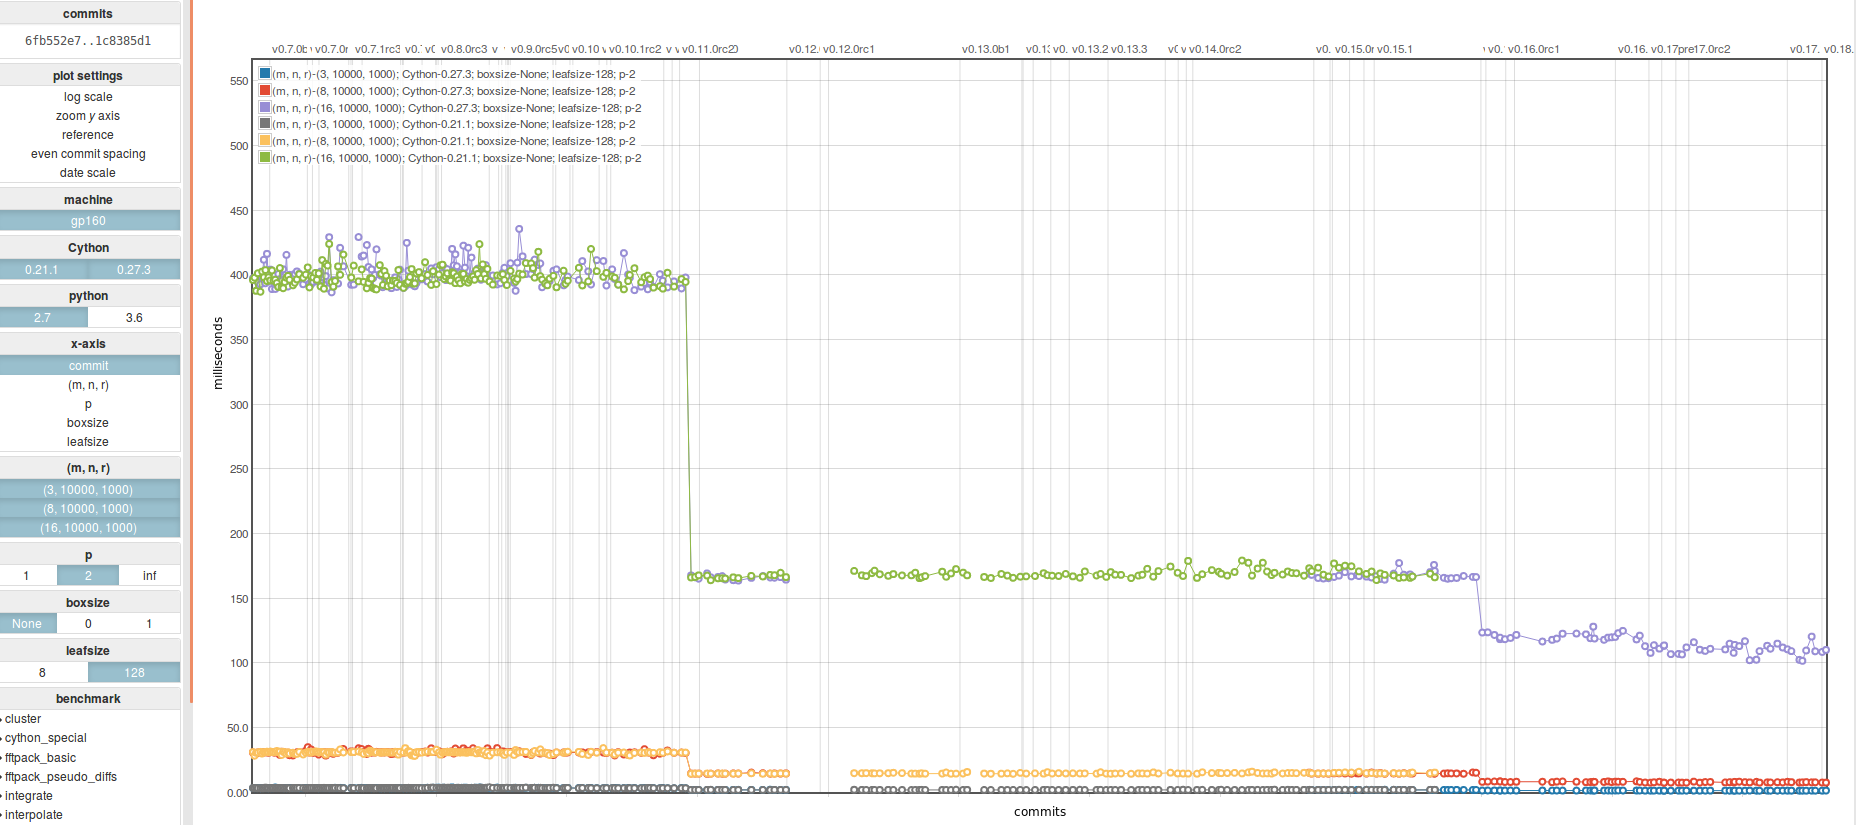
\includegraphics[width=\textwidth]{static/asv_time_query_ckdtree}
        \caption{Airspeed velocity benchmarks for scipy.spatial.cKDTree.query() over a roughly nine year commit history time frame. The results are based on Python 2.7 performance on the master branch of the project using numpy 1.8.2 and Cython versions 0.27.3, 0.21.1, and 0.18 (for improved backward compatibility). Only the L2 (Euclidean) norm is shown here, and to improve backward compatibility and sampling of the benchmarks there was no application of toroidal topology to the KDTree (boxsize argument was ignored).}
        \label{fig:asvbench}
    \end{figure}

   Any pull request can be compared against the \texttt{master} branch with the command \texttt{asv continuous master new-feature}. This will provide a benchmark against the master branch and the branch a new feature is implemented in. More features are available in the documentation, including arguments to select which benchmarks to run.

    \subsubsection*{Test suite}
    The SciPy test suite is orchestrated by a continuous integration matrix
    that includes posix and Windows (32/64-bit) platforms managed by Travis CI and appveyor,
    respectively. Our tests cover Python versions 2.7, 3.4, 3.5, 3.6, and include
    code linting with pyflakes and pycodestyle. There are more than $13000$ unit
    tests in the test suite, which is written for usage with the pytest runner, and
    with a 76.5 \% coverage of approximately $204000$ lines
    of code. Documentation for the code is automatically built and hosted by the
    CircleCI service to facilitate evaluation of documentation changes / integrity.
    Our full test suite also passes with PyPy3, a just-in-time compiled version
    of the Python language.
    % NOTE: is there a citation for PyPy?


\section*{Project organisation and community}

\textbf{Governance}

SciPy adopted an official Governance Document on August 3,
2017\cite{SciPyProjectGovernance}.
We have a Benevolant Dictator for Life (BDFL), Pauli Virtanen, leading the
project, following a detailed discussion of the governance model with the
community on the mailing list.  In practice, the overruling authority of the BDFL
is anticipated to be used only when the Steering Council cannot agree on a matter.
The BDFL is expected to consider any strong indications that they should step down;
although the BDFL may appoint a successor it is generally expected that the Steering
Council will be consulted on the matter.

The (currently) 18 member Steering Council is chaired by Ralf Gommers and performs a number of
tasks including nominating and voting on new Council Members, and actively
contributing to the progress of the project (could be code review but also
outreach activities, etc.). Generally, 1 year of sustained and substantial
contributions (not restricted to source code contributions) that improve
the project are the prerequiste for nomination of new Council Members. Council
Members do not get special treatment for the vast majority of the day to day
project activities (code submission / review), though it is anticipated that their
experience with the project will serve as helpful guidance in many matters.
Council Members have commit rights to the project, but will typically only
incorporate changes when there are no substantive community objections. The
Chair of the Steering Council is responsible for starting more formal
technical reviews of the direction of the project, ensuring that the
composition of the Council remains current, and communicating / summarizing
any Council activities performed privately to the broader community. We also
describe in some detail how institutional partners may contribute to the
project, but no financial weight from grants or other sources
may be leveraged to circumvent or overrule the technical direction of the
project decided upon by the Steering Committee. The Chair does not have
a fixed term, but is nominated by the Steering Committee and is expected
to yield to substantive claims that stepping down is the appropriate action.

SciPy adopted an official Code of Conduct on October 24, 2017
\cite{SciPyCodeOfConduct}, drawing
inspiration from the Apache Foundation Code of
Conduct\cite{ApacheCodeOfConduct}, the Contributor Covenant
\cite{ContributorConvenant},
the Jupyter Code of Conduct \cite{Jupyter_COC}, and the Open Source Guides -
Code of Conduct\cite{OSG_COC}. In short,
we stated five specific guidelines: \emph{be open} (to anyone participating in our community),
\emph{be empathetic and patient} (in resolving conflicts), \emph{be collaborative} (we depend
on each other to build up the tools in the library), \emph{be inquisitive} (identifying issues
early on can be helpful to everyone), and \emph{be careful with wording} (do not harass or exclude).
We outlined a broad diversity inclusion statement, and provide
instructions for contacting the three members of our Code of Conduct Committee or an
external representative on the NumFOCUS Board of Directors.

\textbf{Roadmap}

\textbf{Community beyond the SciPy library}

\textbf{Maintainers and contributors}


\section*{Discussion}

\textit{The Discussion should be succinct and must not contain subheadings.}

\textbf{Impact now}
SciPy has a strong developer community and a massive user base. GitHub
traffic metrics report roughly 20,000 unique visitors to the source
website between May 14 and May 27, 2018, with 721 unique copies (``clones")
of the code base over that roughly two-week period. The developer community
consists of 610 unique contributors of source code, with $>19,000$ commits
accepted into the code base (GitHub page data).

% need some better usage stats sources?
% SciPy stuff from njs blog: https://docs.google.com/spreadsheets/d/1lOLvSF0up4eZyv2ugZi-TM_GIs3gPCkGNIDKXS1Y3w4/edit#gid=406031940
From the user side, there have been at least 15 million downloads
of the SciPy manylinux wheels between the start of 2016 and May of 2018
(njs blog). The recommended source for citing SciPy is simply a reference
to the website / library itself\cite{SciPylib}, and has been cited $>3000$
times. Some of the most prominent citing articles include the IPython
publication\cite{PER-GRA:2007}, a heavily-cited Nature Biotechnology
article\cite{pmid17287757}, a dark
matter annihilitation study in the field of
cosmology\cite{1475-7516-2012-08-007}, and many of the
other major downstream software libraries in the Python scientific
computing stack.

\textbf{Future development}.
\textit{This section should include key issues: sparse arrays, ndimage pixel vs point, splines, fftpack vs. np.fft and linalg vs. np.linalg, under-maintained submodules.}


\bibliography{references}

\noindent Use the cite command for an inline citation, e.g. \cite{behnel2011cython}.

\section*{Acknowledgements (not compulsory)}

Acknowledgements should be brief, and should not include thanks to anonymous referees and editors, or effusive comments. Grant or contribution numbers may be acknowledged.

\section*{Author contributions statement}

Must include all authors, identified by initials, for example:
A.A. conceived the experiment(s),  A.A. and B.A. conducted the experiment(s), C.A. and D.A. analysed the results.  All authors reviewed the manuscript.

\section*{Additional information}

To include, in this order: \textbf{Accession codes} (where applicable); \textbf{Competing financial interests} (mandatory statement).

The corresponding author is responsible for submitting a \href{http://www.nature.com/srep/policies/index.html#competing}{competing financial interests statement} on behalf of all authors of the paper. This statement must be included in the submitted article file.

\end{document}

%%% Local Variables:
%%% mode: latex
%%% TeX-master: t
%%% End:
